\pagebreak
\subsection{Specifica componenti Model::Util}
\label{specificaUtil}
\begin{figure}[!h]
\centering
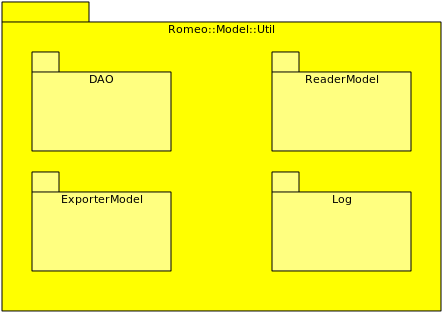
\includegraphics[scale=1]{../Specifica_Tecnica/Content/Immagini/Romeo__Model__Util.png}
			\caption{Diagramma package \textsl{Romeo::Model::Util}}
			\label{comp_romeo::model::util}
\end{figure}
Componente che contiene le classi di supporto per alcune operazioni del core.
%%%%%%%%%%%%%%%%%%%%
%     PACKAGE LOG
%%%%%%%%%%%%%%%%%%%%%%%
\subsection{Specifica componenti Model::Util::Log}
\label{specificaLog}
\begin{figure}[!h]
\centering
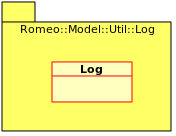
\includegraphics[scale=1]{../Specifica_Tecnica/Content/Immagini/Romeo__Model__Util__Log.png}
			\caption{Diagramma package \textsl{Romeo::Model::Util::Log}}
			\label{comp_romeo::model::util::log}
\end{figure}
Package\g{} che contiene la classe log.
%%%%%%%%%%%%%%%%%%%%
%     CLASSE LOG
%%%%%%%%%%%%%%%%%%%%%%%
\subsubsection{Log (class)}
\label{spelog}
\begin{figure}[!h]
\centering
			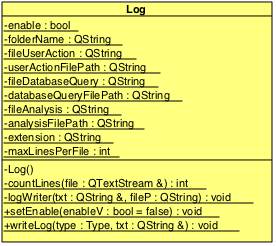
\includegraphics[scale=0.75]{./Content/Immagini/model/Log.png}
			\caption{Diagramma classe \textsl{Log}}
			\label{cl_log}
\end{figure}
\paragraph{Descrizione \\}
Classe utilizzata per la creazione di file di log contenenti i dettagli delle operazioni effettuate in \project{}.
\paragraph{Utilizzo\\}
La classe è utilizzata ad ogni operazioni effettuata dall'utente e ad ogni operazione eseguita sul DAO, essa genera differenti file di log, a seconda delle operazioni che memorizza.
\paragraph{\color{black}Attributi \\}
	\begin{itemize}
		\item \color{teal}\verb! - folderName : static QString !
		\color{black}
		\subparagraph{Descrizione:} stringa che identifica il nome della cartella in cui creare i file di log.
		
		\item \color{teal}\verb! - enable : static boolean!
		\color{black}
		\subparagraph{Descrizione:} attributo che indica se è abilitata o meno  la scrittura del log.
		
		\item \color{teal}\verb! - fileUserAction : static QString !
		\color{black}
		\subparagraph{Descrizione:} indica il nome del file di log contenente le informazioni riguardo alle operazioni utente.
		
		\item \color{teal}\verb! - userActionFilePath : static QString !
		\color{black} 
		\subparagraph{Desrizine: } indica il path del file di log, compreso il nome del file, definito dall'attributo fileUserAction.
		
		\item \color{teal}\verb! - fileDatabaseQuery : static QString !
		\color{black} 
		\subparagraph{Descrizione:} indica il nome del file di log contenente le informazioni riguardanti le operazioni effettuate sul database.
		
		\item \color{teal}\verb!- databaseQueryFilePath : static QString !
		\color{black} 
		\subparagraph{Descrizione:} indica il path del file di log, compreso il nome del file, definito dall'attributo fileDatabaseQuery.
	
		\item \color{teal}\verb! - fileAnalysis : static QString !
		\color{black} 
		\subparagraph{Descrizione:} indica il nome del file di log contenente le informazioni riguardanti le operazioni effettuate durante un'analisi.
	
		\item \color{teal}\verb! - extension : static QString !
		\color{black} 
		\subparagraph{Descrizione:} indica l'estensione dei file di log.
		
		\item \color{teal}\verb! - analysisFilePath : static QString!
		\color{black}
		\subparagraph{Descrizione:} indica il path del file di log, compreso il nome del file, definito dall'attributo fileAnalysis.
		
		\item\color{teal}\verb!- maxLinesPerFile : static QString !
		\color{black} 
		\subparagraph{Descrizione:} indica il numero massimo di linee di testo contenute in un file di log.  Una volta superato tale valore, il contenuto del file corrente viene copiato in un altro, cosi da poterlo svuotare.		
	\end{itemize}


\paragraph{\textcolor{black}{Metodi\\}}
	\begin{itemize}
		\item \color{blue}\verb!- Log()!
		\color{black}
		\subparagraph{Descrizione:} costruttore privato.
		
		\item \color{blue}\verb! +static void setEnable(enableV : boolean)!\\
		\color{black}
		\subparagraph{Descrizione:} metodo che cambia lo stato del Log. Lo abilità o lo disabilità.
		\subparagraph{Argomenti}
			\begin{itemize}
				\item \color{RoyalPurple}\verb!enableV : boolean!\\
				\color{black}Abilita o disabilita il Log.
			\end{itemize}
		\subparagraph{Note}
					\begin{itemize}
						\item Il metodo deve essere marcato statico.
					\end{itemize}
			
		\item \color{blue}\verb! + static void writeLog(type : Type, txt : const QString&)!\\
		\color{black}
		\subparagraph{Decrizione:} metodo che scrive testo su un file.
		\subparagraph{Argomenti}
			\begin{itemize}
				\item \color{blue}\verb!type : Type!\\
				\color{black}Tipo di log che si vuole generare;
				
				\item \color{blue}\verb! txt : const QString&!\\
				\color{black}Testo che va scritto nel log.
			\end{itemize}
		\subparagraph{Note}
					\begin{itemize}
						\item Il metodo deve essere marcato statico.
					\end{itemize}
			
		\item \color{blue}\verb!- static countLines(file : QTextStream &): int!
		\color{black}
		\subparagraph{Descrizione:} metodo che conta le linee presenti nel parametro file.
		\subparagraph{Argomenti}	
			\begin{itemize}
				\item \color{RoyalPurple}\verb!file : QTextStream &!\\
				\color{black}File di cui si vogliono testare le linee.
			\end{itemize}
		\subparagraph{Note}
					\begin{itemize}
						\item Il metodo deve essere marcato statico.
					\end{itemize}
			
		\item \color{blue}\verb! - static logWriter(txt : const QString&, fileP : QString) : void!\\
		\color{black}
		\subparagraph{Descrizione:} metodo che scrive testo su un  file.
		\subparagraph{Argomenti}
			\begin{itemize}
				\item \color{RoyalPurple}\verb!txt : const QString&!\\
				\color{black}Testo da scrivere nel file;
				
				\item \color{RoyalPurple}\verb!fileP : QString!\\
				\color{black}Percorso del file.
			\end{itemize}
		\subparagraph{Note}
			\begin{itemize}
				\item Il metodo deve essere marcato statico.
			\end{itemize}
		
		
	\end{itemize}


%%%%%%%%%%%%%%%%%%%%
%     PACKAGE READERMODEL
%%%%%%%%%%%%%%%%%%%%%%%
\color{black}
\subsection{Specifica componenti Model::Util::ReaderModel}
\label{specificaReaderModel}
\begin{figure}[!h]
\centering
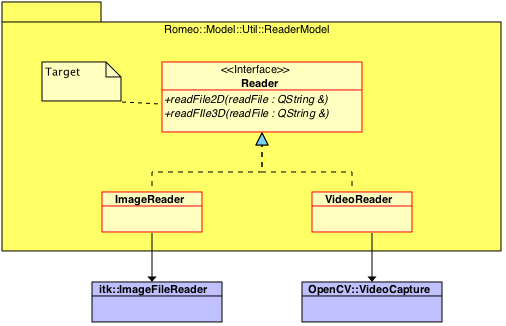
\includegraphics[scale=0.8]{../Specifica_Tecnica/Content/Immagini/Romeo__Model__Util__ReaderModel.png}
			\caption{Diagramma package \textsl{Romeo::Model::Util::ReaderModel}}
			\label{comp_romeo::model::util::readermodel}
\end{figure}
Componente che contiene le classi utilizzate per leggere i vari formati di immagini su cui opera \project.

\pagebreak
%%%%%%%%%%%%%%%%%%%%
%     INTERFACCIA READER
%%%%%%%%%%%%%%%%%%%%%%%
\subsubsection{Reader (interface)}
\label{spereader}
\begin{figure}[!h]
\centering
			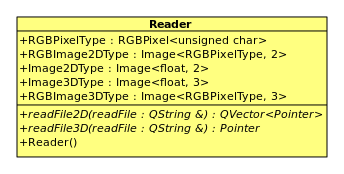
\includegraphics[scale=5]{./Content/Immagini/model/Reader.png}
			\caption{Interfaccia Reader: metodi}
			\label{cl_reader}
\end{figure}
\paragraph{Descrizione \\}
L'interfaccia rappresenta un generico oggetto reader, essa fornisce il contratto ai reader concreti.
\paragraph{Utilizzo\\}
L'interfaccia fornisce dei contratti puri che saranno implementati dalle sottoclassi.

\paragraph{\textcolor{black}{Metodi\\}}
%READFILE2D
\color{blue}\verb!+ readFile2D(readFile : QString &): RGBImage2DType::Pointer!
\begin{quote}
\color{black} Metodo virtuale puro che ha come contratto la lettura di un file 2D. Il metodo deve essere ridefinito dalle classi che ereditano da questa, definendo la lettura di un file 2D.

\textbf{Argomenti}
\begin{itemize}
\item \verb!readFile : QString &! \\ Riferimento al nome del file che il metodo deve leggere.
\end{itemize}

\textbf{Note}
\begin{itemize}
\item questo metodo deve essere marcato virtuale puro;
\item questo metodo deve essere ridefinito.
\end{itemize}
\end{quote} 
%READFILE3D
\color{blue}\verb!+ readFil32D(readFile : QString &): RGBImage3DType::Pointer!
\begin{quote}
\color{black} Metodo virtuale puro che ha come contratto la lettura di un file 3D. Il metodo deve essere ridefinito dalle classi che ereditano da questa, definendo la lettura di un file 3D.

\textbf{Argomenti}
\begin{itemize}
\item \verb!readFile : QString &! \\ Riferimento al nome del file che il metodo deve leggere.
\end{itemize}

\textbf{Note}
\begin{itemize}
\item questo metodo deve essere marcato virtuale puro;
\item questo metodo deve essere ridefinito.
\end{itemize}
\end{quote} 

\color{black}
%%%%%%%%%%%%%%%%%%%%
%     CLASSE IMAGEREADER
%%%%%%%%%%%%%%%%%%%%%%%
\pagebreak
\subsubsection{ImageReader (class)}
\label{speimagereader}
\begin{figure}[!h]
\centering
			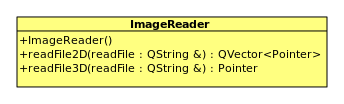
\includegraphics[scale=5]{./Content/Immagini/model/ImageReader.png}
			\caption{Classe ImageReader: attributi e metodi}
			\label{cl_imagereader}
\end{figure}
\paragraph{Descrizione \\}
Classe che rappresenta l'oggetto incaricato di caricare file di tipo 2D e 3D non time-dipendent.
\paragraph{Utilizzo\\}
La classe implementerà i metodi virtuali puri della superclasse.
\paragraph{Classi ereditate\\}
\begin{itemize}
\item \hyperref[spereader]{Reader}.
\end{itemize}
\paragraph{\color{black}Attributi \\}
%FOLDERNAME
\color{teal}\verb!- itk::ImageFileReader reader!
\begin{quote}
\color{black}Oggetto del toolkit itk che identifica un reader per la lettura di file di tipo immagine dal file system.
\end{quote}
\paragraph{\textcolor{black}{Metodi\\}}
%costruttore
\color{blue}\verb!+ ImageReader()!
\begin{quote}
\color{black}Costruttore pubblico della classe ImageReader.
\end{quote}
%READFILE2D

\color{blue}\verb!+ readFile2D(readFile : QString &): RGBImage2DType::Pointer!
\begin{quote}
\color{black} Metodo che implementa il contratto fornito dalla classe astratta \hyperref[spereader]{Reader}.

\textbf{Argomenti}
\begin{itemize}
\item \verb!readFile : QString &! \\ Riferimento al nome del file che il metodo deve leggere.
\end{itemize}

\textbf{Note}
\begin{itemize}
\item questo metodo deve essere marcato virtuale;
\item questo metodo è stato ridefinito.
\end{itemize} 
\end{quote}
%READFILE3D
\color{blue}\verb!+ readFile3D(readFile : QString &): RGBImage3DType::Pointer!
\begin{quote}
\color{black} Metodo che implementa il contratto fornito dalla classe astratta \hyperref[spereader]{Reader}.

\textbf{Argomenti}
\begin{itemize}
\item \verb!readFile : QString &! \\ Riferimento al nome del file che il metodo deve leggere.
\end{itemize}

\textbf{Note}
\begin{itemize}
\item questo metodo deve essere marcato virtuale;
\item questo metodo è stato ridefinito.
\end{itemize}
\end{quote} 

\color{black}
%%%%%%%%%%%%%%%%%%%%
%     CLASSE VIDEOREADER
%%%%%%%%%%%%%%%%%%%%%%%
\pagebreak

\subsubsection{VideoReader (class)}
\label{spevideoreader}
\begin{figure}[!h]
\centering
			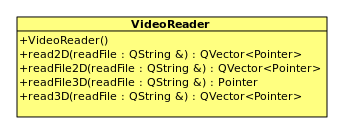
\includegraphics[scale=5]{./Content/Immagini/model/VideoReader.png}
			\caption{Classe VideoReader: attributi e metodi}
			\label{cl_videoreader}
\end{figure}
\paragraph{Descrizione \\}
Classe che rappresenta l'oggetto incaricato di caricare file di tipo 2D e 3D time-dipendent.
\paragraph{Utilizzo\\}
La classe implementerà i metodi virtuali puri della superclasse \hyperref[spereader]{Reader}.
\paragraph{Classi ereditate\\}
\begin{itemize}
\item \hyperref[spereader]{Reader}.
\end{itemize}
\paragraph{\color{black}Attributi \\}
%FOLDERNAME
\color{teal}\verb!- itk::VideoFileReader reader!
\begin{quote}
\color{black}Oggetto del toolkit itk che identifica un reader per la lettura di file di tipo video dal file system.
\end{quote}
\paragraph{\textcolor{black}{Metodi\\}}
%costruttore
\color{blue}\verb!+ VideoReader()!
\begin{quote}
\color{black}Costruttore pubblico della classe VideoReader. \\
\end{quote}
%READFILE2D
\color{blue}\verb!+ readFile2D(readFile : QString &): RGBImage2DType::Pointer!
\begin{quote}
\color{black} Metodo che implementa il contratto fornito dalla classe astratta \hyperref[spereader]{Reader}.

\textbf{Argomenti}
\begin{itemize}
\item \verb!readFile : QString &! \\ Riferimento al nome del file che il metodo deve leggere.
\end{itemize}

\textbf{Note}
\begin{itemize}
\item questo metodo deve essere marcato virtuale;
\item questo metodo è stato ridefinito.
\end{itemize}
\end{quote} 
%READFILE3D
\color{blue}\verb!+ readFile3D(readFile : QString &): RGBImage3DType::Pointer!
\begin{quote}
\color{black} Metodo che implementa il contratto fornito dalla classe astratta \hyperref[spereader]{Reader}.

\textbf{Argomenti}
\begin{itemize}
\item \verb!readFile : QString &! \\ Riferimento al nome del file che il metodo deve leggere.
\end{itemize}

\textbf{Note}
\begin{itemize}
\item questo metodo deve essere marcato virtuale;
\item questo metodo è stato ridefinito.
\end{itemize}
\end{quote} 
\color{black}


%%%%%%%%%%%%%%%%%%%%
%     PACKAGE EXPORTERMODEL
%%%%%%%%%%%%%%%%%%%%%%%
\subsection{Specifica componenti Model::Util::ExporterModel}
\label{specificaExporterModel}
\begin{figure}[!h]
\centering
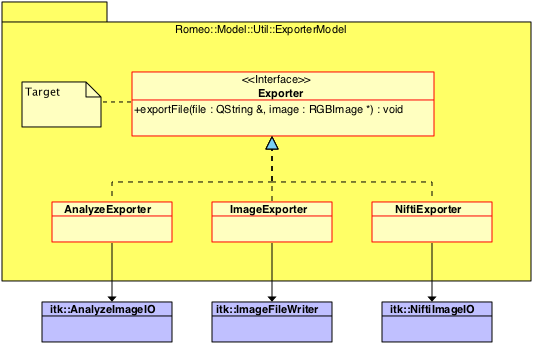
\includegraphics[scale=0.8]{../Specifica_Tecnica/Content/Immagini/Romeo__Model__Util__ExporterModel.png}
			\caption{Diagramma package \textsl{Romeo::Model::Util::ExporterModel}}
			\label{comp_romeo::model::util::exporterrmodel}
\end{figure}
Package\g{} che contiene le classi utilizzate per esportare in vari formati i risultati delle analisi effettuati da \project.

%%%%%%%%%%%%%%%%%%%%
%     INTERFACCIA EXPORTER
%%%%%%%%%%%%%%%%%%%%%%%
\pagebreak
\subsubsection{Exporter (interface)}
\label{spexporter}
\begin{figure}[!h]
\centering
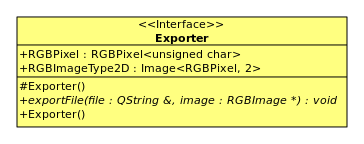
\includegraphics[scale=5]{./Content/Immagini/model/Exporter.png}
			\caption{Diagramma classe \textsl{Exporter}}
			\label{cl_exporter}
\end{figure}
\paragraph{Descrizione \\}
L'interfaccia rappresenta un generico oggetto exporter, essa fornisce il contratto alle classi exporter concrete.
\paragraph{Utilizzo\\}
L'interfaccia fornisce dei contratti puri che saranno implementati dalle sottoclassi.
\paragraph{\textcolor{black}{Metodi\\}}
	\begin{itemize}

%READFILE2D

		\item \color{blue}\verb!+ exportImage(file : QString &, image: RGBImage*)!
		\subparagraph{Descrizione:} Metodo virtuale puro che ha come contratto la scrittura di un oggetto di tipo RGBImage su file system con il nome contenuto nel parametro file.
\color{black}
		\subparagraph{Argomenti}
			\begin{itemize}
				\item \color{RoyalPurple}\verb!file : QString &! \\ 
				\color{black}Riferimento al nome che il metodo deve dare al file che scriverà nel file system.
				\item \color{RoyalPurple}\verb!image : RGBImage*! \\ 
				\color{black}Puntatore all'oggetto che rappresenta l'immagine che il metodo deve scrivere su file system
			\end{itemize}
\color{black}
		\subparagraph{Note}
			\begin{itemize}
				\item questo metodo deve essere marcato virtuale puro;
				\item questo metodo deve essere ridefinito.
			\end{itemize}
	\end{itemize}
		\color{black}

\pagebreak
%%%%%%%%%%%%%%%%%%%%
%     CLASSE EXPORTER2D
%%%%%%%%%%%%%%%%%%%%%%%
\subsubsection{Exporter2D (class)}
\label{spexporter2d}
\begin{figure}[!h]
\centering
			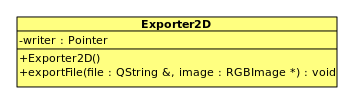
\includegraphics[scale=5]{./Content/Immagini/model/Exporter2D.png}
			\caption{Diagramma classe \textsl{Exporter2D}}
			\label{cl_exporter2d}
\end{figure}

\paragraph{Descrizione \\}
Classe che rappresenta l'oggetto incaricato di scrivere sul disco le immagini 2D elaborate in \project.
\paragraph{Utilizzo\\}
La classe implementerà i metodi virtuali puri della superclasse.
\paragraph{Classi ereditate\\}
\begin{itemize}
\item \hyperref[spexporter]{Exporter}.
\end{itemize}
\paragraph{\color{black}Attributi \\}
	\begin{itemize}
%FOLDERNAME
		\item \color{teal}\verb!- itk::ImageFileWriter writer!
		\color{black}
		\subparagraph{Descrizione:} Oggetto del toolkit itk che identifica un writer per la scrittura di file di tipo immagine 2D nel file system.
	\end{itemize}	
\paragraph{\textcolor{black}{Metodi}}
	\begin{itemize}
%costruttore
		\item \color{blue}\verb!+ Export2D()!
		\color{black}
		\subparagraph{Descrizione:} Costruttore pubblico della classe Export2D.

%READFILE2D

		\item \color{blue}\verb!+ ExportFileconst (file: QString&, image: RGBImage*): void RGBImage2DType::Pointer!
		\color{black}
		\subparagraph{Descrizione:} Metodo che implementa il contratto fornito dalla classe astratta \hyperref[spexporter]{Exporter}. Esso scrive su disco l'immagine rappresentata dal parametro image di tipo puntatore ad RGBImage nel percorso indicato dal parametro file di tipo riferimento a QString.

		\subparagraph{Argomenti}
			\begin{itemize}
				\item \color{RoyalPurple}\verb!file : QString &! \\ 
				\color{black}Riferimento al nome che l'immagine scritta sul disco dovrà avere.
				\item \color{RoyalPurple}\verb!image : RGBImage*! \\ 
				\color{black}Puntatore all'oggetto rappresentante l'immagine che dovrà essere scritta su disco.
			\end{itemize}
\color{black}
		\subparagraph{Note}
			\begin{itemize}
				\item questo metodo deve essere marcato virtuale;
				\item questo metodo deve essere marcato costante;
				\item questo metodo è stato ridefinito.
			\end{itemize} 
	\end{itemize}
\color{black}

%%%%%%%%%%%%%%%%%%%%
%     CLASSE EXPORTER3D
%%%%%%%%%%%%%%%%%%%%%%%
\pagebreak
\subsubsection{Exporter3D (class)}
\label{spexporter3d}
\begin{figure}[!h]
\centering
			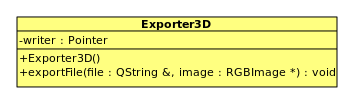
\includegraphics[scale=5]{./Content/Immagini/model/Exporter3D.png}
			\caption{Diagramma classe \textsl{Exporter3D}}
			\label{cl_exporter3d}
\end{figure}
\paragraph{Descrizione \\}
Classe che rappresenta l'oggetto incaricato di scrivere sul disco le immagini 3D elaborate in \project.
\paragraph{Utilizzo\\}
La classe implementerà i metodi virtuali puri della superclasse.
\paragraph{Classi ereditate\\}
\begin{itemize}
\item \hyperref[spexporter]{exporter}.
\end{itemize}
\paragraph{\color{black}Attributi \\}
	\begin{itemize}
%FOLDERNAME
		\item \color{teal}\verb!- itk::ImageFileWriter writer!
		\color{black}
		\subparagraph{Descrizione:} Oggetto del toolkit itk che identifica un writer per la scrittura di file di tipo immagine 3D nel file system.
	\end{itemize}
\paragraph{\textcolor{black}{Metodi}}
	\begin{itemize}
%costruttore
		\item \color{blue}\verb!+ Export3D()!
		\color{black}
		\subparagraph{Descrizione:} Costruttore pubblico della classe Export3D.

%READFILE2D

		\item\color{blue}\verb!+ ExportFileconst (file: QString&, image: RGBImage*): void RGBImage2DType::Pointer!
		\color{black}
		\subparagraph{Descrizione:} Metodo che implementa il contratto fornito dalla classe astratta \hyperref[spexporter]{Exporter}. Esso scrive su disco l'immagine rappresentata dal parametro image di tipo puntatore ad RGBImage nel percorso indicato dal parametro file di tipo riferimento a QString.

		\subparagraph{Argomenti}
			\begin{itemize}
				\item \color{RoyalPurple}\verb!file : QString &! \\ 
				\color{black}Riferimento al nome che l'immagine scritta sul disco dovrà avere.
				\item \color{RoyalPurple}\verb!image : RGBImage*! \\ 
				\color{black}Puntatore all'oggetto rappresentante l'immagine che dovrà essere scritta su disco.
			\end{itemize}
\color{black}
		\subparagraph{Note}
			\begin{itemize}
				\item questo metodo deve essere marcato virtuale;
				\item questo metodo deve essere marcato costante;
				\item questo metodo è stato ridefinito.
			\end{itemize} 
	\end{itemize}
\color{black}

%%%%%%%%%%%%%%%%%%%%
%     PACKAGE DAO
%%%%%%%%%%%%%%%%%%%%%%%
\pagebreak
\subsection{Specifica componenti Model::Util::DAO}
\label{specificaDAO}
\begin{figure}[!h]
\centering
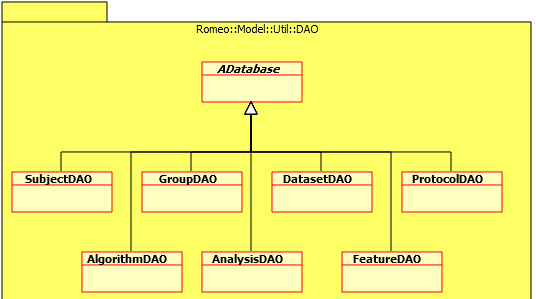
\includegraphics[scale=0.8]{../Specifica_Tecnica/Content/Immagini/Romeo__Model__Util__DAO.png}
			\caption{Diagramma package \textsl{Romeo::Model::Util::DAO}}
			\label{comp_romeo::model::util::dao}
\end{figure}
Package\g{} che contiene le classi per l'interazione di \project con il Database.

\color{black}

\pagebreak
%%%%%%%%%%%%%%%%%%%%
%     CLASSE ADATABASE
%%%%%%%%%%%%%%%%%%%%%%%
\subsubsection{ADatabase (Abstract)}
\label{speadatabase}
\begin{figure}[!h]
\centering
			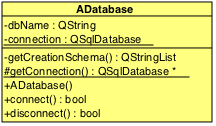
\includegraphics[scale=1]{./Content/Immagini/model/ADatabase.png}
			\caption{Diagramma classe \textsl{ADatabase}}
			\label{cl_adatabase}
\end{figure}

\paragraph{Descrizione \\}
Classe astratta che fornisce i metodi di connessione e disconnessione al database e dei metodi per notificare eventuali errori dovuti al collegamento con componenti esterne, nel nostro caso, il database. Tale classe viene solamente estesa dalle classi che opereranno sulle tabelle del database.

\paragraph{Utilizzo\\}
La classe viene creata alla creazione di una sua sottoclasse.

\paragraph{Eredita da:}
	\begin{itemize}
		\item Qt::QSqlDatabase.
	\end{itemize}
	
\paragraph{\color{black}Attributi \\}
	\begin{itemize}
		\item \color{teal}\verb! - static connection : QSqlDatabase!\\
		\color{black}
		\subparagraph{Descrizione:} attributo statico che identifica la connessione ad un database.
		
		\item \color{teal}\verb! -dbName : QString!\\
		\color{black}
		\subparagraph{Descrizione:} nome del database a qui si è connesso.
		
	\end{itemize}

\paragraph{\textcolor{black}{Metodi}}
\begin{itemize}
	\item \color{blue}\verb! -getCreationSchema() : QStringList!\\
	\color{black}
	\subparagraph{Descrizione:} metodo che ritorna lo schema SQL del dtabase.
	
	\item \color{blue}\verb! # static getConnection() : QSqlDatabase *!\\
	\color{black}
	\subparagraph{Descrizione:} metodo che si occupa di creare la connessione al database.
	
	\item \color{blue}\verb! + ADatabase()!\\
	\color{black}
	\subparagraph{Descrizione:} costruttore delle classe. Esso controlla se l'attributo \verb!connection! contiene già una connesione, in caso negatiovo la crea.
	
	\item \color{blue}\verb! + connect() : boolean!\\
	\color{black}
	\subparagraph{Descrizione:} metodo pubblico che effettua la connessione al database e ritorna se questa è stata effettuata con successo.

	\item \color{blue}\verb! + disconnect() : boolean!\\
	\color{black}
	\subparagraph{Descrizione:} metodo che effettua la disconnessione dal database e ritorna se questa è stata effettuata con successo.
	
\end{itemize}

\pagebreak
%%%%%%%%%%%%%%%%%%%%
%     CLASSE ALGORITHMDAO
%%%%%%%%%%%%%%%%%%%%%%%

\subsubsection{AlgorithmDAO(class)}
\label{spealgorithmdao}
\begin{figure}[!h]
\centering
			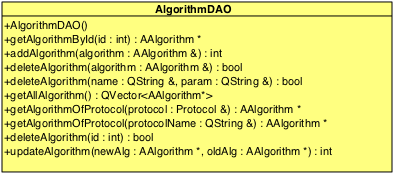
\includegraphics[scale=1]{./Content/Immagini/model/AlgorithmDAO.png}
			\caption{Diagramma classe \textsl{AlgorithmDAO}}
			\label{cl_algorithmdao}
\end{figure}

\paragraph{Descrizione \\}
Classe che rappresenta l'oggetto incaricato di operare con la tabella Algorithm del database.
\paragraph{Utilizzo\\}
La classe verrà utilizzata dal core quando dovrà salvare nel database, o recuperare da esso informazioni riguardanti gli algoritmi creati dall'utente o utilizzati da\project.

\paragraph{Classi ereditate\\}
	\begin{itemize}
		\item \hyperref[speadatabase]{Romeo::Model::Util::DAOADatabase}.
	\end{itemize}
\paragraph{\textcolor{black}{Metodi\\}}
	\begin{itemize}
		\item \color{blue}\verb!+ AlgorithmDAO()!\\
		\color{black}
		\subparagraph{Descrizione:} costruttore della classe \textsl{AlgorithmDAO}, richiama il costruttore della superclasse.
		
		%GETALGORITHMBYID
		\item \color{blue}\verb! + getAlgorithmById(id : const int): AAlgorithm*!\\
		\color{black}
		\subparagraph{Descrizione:} metodo pubblico che ricerca all'interno del database un algoritmo avente l'id indicato nel parametro. Esso ritorna un puntatore a tale algoritmo di tipo \textsl{AAlgorithm}.
		\subparagraph{Argomenti}
			\begin{itemize}
				\item \color{RoyalPurple}\verb!id : const int! \\
				\color{black}Indica l'id dell'algoritmo da cercare.
			\end{itemize}
			
		%ADDALGORITHM
		\item \color{blue}\verb!+ addAlgorithm(algorithm : const AAlgorithm*): QVariant!\\
		\color{black}
		\subparagraph{Descrizione:} metodo pubblico che aggiunge nel database un nuovo algoritmo passato come parametro. Esso ritorna l'ultimo id creato nella tabella Algorithm del database.
		\subparagraph{Argomenti}
			\begin{itemize}
				\item \color{RoyalPurple} \verb!algorithm : AAlgorithm*! \\
				\color{black} Puntatore all'oggetto di tipo \textsl{AAlgorithm} da inserire nel database.
			\end{itemize}
			
		%DELETEALGORITHM
		\item \color{blue}\verb!+ deleteAlgorithm(algorithm :  AAlgorithm*) : boolean!\\
		\color{black} 
		\subparagraph{Descrizione:} metodo pubblico che rimuove dal database un algoritmo passato come parametro.
		\subparagraph{Argomenti}
			\begin{itemize}
				\item \color{RoyalPurple}\verb!algorithm :  AAlgorithm*! \\ 
				\color{black}Puntatore all'oggetto di tipo \textsl{AAlgorithm} da eliminare dal database.
			\end{itemize}
		
		%DELETEALGORITHM
		\item \color{blue}\verb!+ deleteAlgorithm(name : const QString &, param: const QString &) : boolean!\\
		\color{black} 
		\subparagraph{Descrizione:} metodo pubblico che rimuove dal database un algoritmo avente nome e parametri passati come parametro.
		\subparagraph{Argomenti}
			\begin{itemize}
				\item \color{RoyalPurple}\verb!name : const QString &! \\ 
				\color{black}Riferimento alla stringa avente il nome dell'algoritmo da eliminare.
				\item \color{RoyalPurple}\verb!param : const QString &! \\ 
				\color{black}Riferimento alla stringa avente tutti i parametri dell'algoritmo che si vuole eliminare.
			\end{itemize}
			
		%GETALLALGORITHM
		\item \color{blue}\verb!+ getAllAlgorithm(): QVector<AAlgorithm *>!
		\color{black}
		\subparagraph{Descrizione:} metodo pubblico che ritorna un \textsl{QVector} di puntatori ad oggetti di tipo \textsl{AAlgorithm} contenente tutti gli algoritmi presenti nel database.
		
		%GETALGORITHMOFPROTOCOL
		\item \color{blue}\verb!+ getAlgorithmOfProtocol(protocol : const Protocol &): AAlgorithm *!\\
		\color{black} 
		\subparagraph{Descrizione:} metodo pubblico che ritorna un puntatore all'oggetto AAlgorithm, che rappresenta l'algoritmo che fa parte del protocol passato come parametro.
		\subparagraph{Argomenti}
			\begin{itemize}
				\item \color{RoyalPurple}\verb!protocol : const Protocol &! \\ 
				\color{black}Riferimento al \textsl{Protocol} del quale si vuole ricavare l'algoritmo.
			\end{itemize}

		%GETALGORITHMOFPROTOCOL
		\item \color{blue}\verb!+ getAlgorithmOfProtocol(protocolName : const QString &): AAlgorithm*!\\
		\color{black} 
		\subparagraph{Descrizione:} metodo pubblico che ritorna un puntatore all'oggetto \textsl{AAlgorithm}, che rappresenta l'algoritmo membro del protocol\g{} avente il nome passato come parametro.
		\subparagraph{Argomenti:}
			\begin{itemize}
				\item \color{RoyalPurple}\verb!protocolName : const QString &! \\
				\color{black} Riferimento al nome del Protocol\g{} del quale si vuole ricavare l'algoritmo.
			\end{itemize}
		
		%
		\item \color{blue}\verb! + deleteAlgorithm(id : int) : boolean!\\
		\color{black}
		\subparagraph{Descrizone:} metodo che elimina l'algoritmo dal database.
		\subparagraph{Argomenti}
			\begin{itemize}
				\item \color{RoyalPurple}\verb!id : int!\\
				\color{black}Id dell'algoritmo che si vuole eliminare.
			\end{itemize}
			
		\item \color{blue}\verb! + updateAlgorithm(newAlg : AAlgorithm *, oldAlg : AAlgorithm *) : int!\\
		\color{black}
		\subparagraph{Descrizione:} metodo che sostituisce un algoritmo\g{}. Ritorna l'id del nuovo algoritmo.
		\subparagraph{Argomenti}
			\begin{itemize}
				\item \color{RoyalPurple}\verb!newAlg : AAlgorithm *!\\
				\color{black}Nuovo algoritmo;
				
				\item \color{RoyalPurple}\verb!oldAlg : AAlgorithm *!\\
				\color{black}Vecchio algoritmo da modificare.
			\end{itemize}

	\end{itemize}

\color{black}

\pagebreak
%%%%%%%%%%%%%%%%%%%%
%     CLASSE ANALYSISDAO
%%%%%%%%%%%%%%%%%%%%%%%

\subsubsection{AnalysisDAO(class)}
\label{speanalysisdao}
\begin{figure}[!h]
\centering
			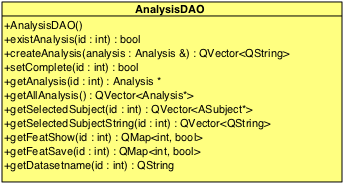
\includegraphics[scale=1]{./Content/Immagini/model/AnalysisDAO.png}
			\caption{Diagramme classe \textsl{AnalysisDAO}}
			\label{cl_analysisdao}
\end{figure}

\paragraph{Descrizione \\}
Classe che rappresenta l'oggetto incaricato di operare con la tabella Analysis del database.
\paragraph{Utilizzo\\}
La classe verrà utilizzata dal core quando dovrà salvare nel database, o recuperare da esso informazioni riguardanti le analisi effettuate dall'utente.
\paragraph{Classi ereditate\\}
	\begin{itemize}
	\item \hyperref[speadatabase]{Romeo::Model::Util::DAO::ADatabase}.
	\end{itemize}
	
\paragraph{\textcolor{black}{Metodi\\}}
\begin{itemize}
	\item \color{blue}\verb!+ AnalysisDAO()!\\
	\color{black}
	\subparagraph{Descrizione:} costruttore pubblico che richiama il costruttore della superclasse in modo da stabilire una connessione con il database. 
	
	\item \color{blue}\verb! + existAnalysis(id : int) : boolean!\\
	\color{black}
	\subparagraph{Descrizione:} metodo che controlla se esiste giù un analsi avente l'id passato.
	\subparagraph{Argomenti}
		\begin{itemize}
			\item \color{RoyalPurple}\verb!id : int!\\
			\color{black}Rappresenta l'id dell'oggetto \textsl{Analysis} da cercare.
		\end{itemize}
	
	 %CREATEANALYSIS
	\item \color{blue}\verb! + createAnalysis(analysis : const Analysis &): boolean!\\
	\color{black} 
	\subparagraph{Descrizione:} metodo pubblico che aggiunge nel database informazioni riguardanti l'analisi passata come parametro. Esso ritorna true se l'operazione va a buon fine, false altrimenti.
	\subparagraph{Argomenti}
		\begin{itemize}
			\item \color{RoyalPurple} \verb!analysis : const Analysis &! \\ 
			\color{black}Riferimento all'oggetto di tipo \textsl{Analysis}, le cui informazioni vengono aggiunte al database.
		\end{itemize}
		
	\item \color{blue}\verb! + setComplete(id : int) : boolean!\\
	\color{black}
	\subparagraph{Descrizione:} metodo che assegna il valore di completato all'oggetto \textsl{Analysis} avente l'id passato come argomento.
	\subparagraph{Argomenti}
		\begin{itemize}
			\item \color{RoyalPurple}\verb!id : int!\\
			\color{black}Id dell'analisi a cui assegnare il valore complete.
		\end{itemize}
			
	\item \color{blue}\verb! + getAnalysis(id : int) : Analysis *!\\
	\color{black}
	\subparagraph{Descrizione:} metodo che ritorna un puntatore ad un oggetto \textsl{Analysis}, avente come id il valore passato.
	\subparagraph{Argomenti}
		\begin{itemize}
			\item \color{RoyalPurple}\verb!id : int!\\
			\color{black}Id dell'analisi che si vuole ottenere.
		\end{itemize}
	\subparagraph{Note}
		\begin{itemize}
			\item Il metodo deve essere marcato come costante.
		\end{itemize}
		
	\item \color{blue}\verb! + getAllAnalysis() : QVector<Analysis*>!\\
	\color{black}
	\subparagraph{Descrizione:} metodo che ritorna un vettore contenente tutte le analisi effettuate dall'utente.
	\subparagraph{Note}
			\begin{itemize}
				\item Il metodo deve essere marcato come costante.
			\end{itemize}
			
	\item \color{blue}\verb! + getSelectedSubject(id : int) : QVector<ASubject* >!\\
	\color{black}
	\subparagraph{Descrizione:} metodo che ritorna un vettore contenente i Subject\g{} selezionati nell'analisi avente l'id dato.
	\subparagraph{Argomenti}
		\begin{itemize}
			\item \color{RoyalPurple}\verb!id : int!\\
			\color{black}Id dell'analisi di cui si vogliono conoscere i Subject\g{} selezionati.
		\end{itemize}
	\subparagraph{Note}
		\begin{itemize}
			\item Il metodo deve essere marcato come costante.
		\end{itemize}
		
	\item \color{blue}\verb! + getSelectedSubjectString(id : int) : QVector<QString>!\\
	\color{black}
	\subparagraph{Descrizione:} metodo che ritorna l'elenco dei nomi dei Subject\g{} selezionati dall'utente nell'analisi avente l'id passato.
	\subparagraph{Argomenti}
		\begin{itemize}
			\item \color{RoyalPurple}\verb!id : int!\\
			\color{black}Id dell'analisi di cui si vogliono conoscere i nomi del Subject\g{} selezionati.
		\end{itemize}
	\subparagraph{Note}
		\begin{itemize}
			\item Il metodo deve essere marcato come costante.
		\end{itemize}
		
	\item \color{blue}\verb! + getFeatShow(id : int) : QMap<int, bool>!\\
	\color{black}
	\subparagraph{Descrizione:} metodo che ritorna una mappa contenente per ogni feature un booleano che rappresenta se la feature\g{} è stata mostrata o meno.
	\subparagraph{Argomeni}
		\begin{itemize}
			\item \color{RoyalPurple}\verb!id : int!\\
			\color{black}Id dell'analisi di cui si vogliono ottenere le feature\g{} mostrate.
		\end{itemize}
	\subparagraph{Note}
		\begin{itemize}
			\item Il metodo deve essere marcato come costante.
		\end{itemize}
		
	\item \color{blue}\verb!+getFeatSave(id : int) : QMap<int, bool>!\\
	\color{black}
	\subparagraph{Descrizione:} metodo che ritorna una mappa contenente per ogni feature\g{} un booleano che rappresenta se la feature\g{} è stata salvata o meno.
	\subparagraph{Argomeni}
		\begin{itemize}
			\item \color{RoyalPurple}\verb!id : int!\\
			\color{black}Id dell'analisi di cui si vogliono ottenere le feature\g{} esportate.
		\end{itemize}
	\subparagraph{Note}
		\begin{itemize}
			\item Il metodo deve essere marcato come costante.
		\end{itemize}
		
	\item \color{blue}\verb! + getDatasetname(id : int) : QString!\\
	\color{black}
	\subparagraph{Descrizone:} metodo che ritorna il nome del Dataset\g{} associato all'analisi avente l'id passato.
	\subparagraph{Argomenti}
		\begin{itemize}
			\item \color{RoyalPurple}\verb!id : int!\\
			\color{black}Id dell'analisi di cui si vole ottenere il Dataset\g{}.
		\end{itemize}


\end{itemize}

\pagebreak
%%%%%%%%%%%%%%%%%%%%
%     CLASSE DATASETDAO
%%%%%%%%%%%%%%%%%%%%%%%

\subsubsection{DatasetDAO(class)}
\label{spedatasetdao}
\begin{figure}[!h]
\centering
			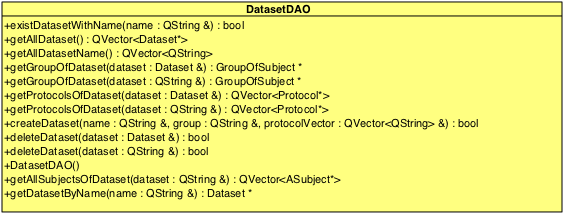
\includegraphics[scale=1]{./Content/Immagini/model/DatasetDAO.png}
			\caption{Classe DatasetDAO: attributi e metodi}
			\label{cl_datasetdao}
\end{figure}
\paragraph{Descrizione \\}
Classe che rappresenta l'oggetto incaricato di operare con la tabella \dataset{} del database.
\paragraph{Utilizzo\\}
La classe verrà utilizzata dal core quando dovrà salvare nel database, o recuperare da esso informazioni riguardanti i \dataset{} creati dall'utente o utilizzati da \project.
\paragraph{Classi ereditate\\}
\begin{itemize}
\item \hyperref[speadatabase]{ADatabase}.
\end{itemize}
\paragraph{\textcolor{black}{Metodi\\}}
%costruttore
\color{blue}\verb!+ DatasetDAO()!
\begin{quote}
\color{black} Costruttore pubblico che richiama il costruttore della superclasse in modo da stabilire una connessione con il database. \\
\end{quote}

%EXISTDATASETWITHNAME
\color{blue}\verb!+ existSubjectWithName(name : const QString &)!
\begin{quote}
\color{black} Metodo pubblico che controlla se all'interno del database è già presente un \dataset{} avente il nome passato come parametro. 

\textbf{Argomenti}
\begin{itemize}
\item \verb!name : const QString &! \\ Riferimento al nome del \dataset{} del quale si vuole verificare l'esistenza.
\end{itemize}
\end{quote}

%GETALLDATASET
\color{blue}\verb!+ getAllDataset(): QVector<Dataset*>!
\begin{quote}
\color{black} Metodo pubblico che ritorna un QVector di puntatori ad oggetti di tipo Dataset, contenente tutti i \dataset{} presenti nel database.
\end{quote}

%GETALLDATASETNAME
\color{blue}\verb!+ getAllDatasetName(): QVector<QString>!
\begin{quote}
\color{black} Metodo pubblico che ritorna un QVector di QString, contenente il nome tutti i \dataset{} presenti nel database.
\end{quote}

%GETGROUPOFDATASET
\color{blue}\verb!+ getGroupOfDataset(dataset : const Dataset &): QVector<GroupOfSubject*>!
\begin{quote}
\color{black} Metodo pubblico che ritorna un QVector di puntatori ad oggetti di tipo GroupOfSubject, contenente tutti i gruppi di \subject{} membri del \dataset{} passato come parametro.

\textbf{Argomenti}
\begin{itemize}
\item \verb!dataset : const Dataset &! \\ Riferimento al  \dataset{} del quale si vogliono ricavare i gruppi membri.
\end{itemize}
\end{quote}

%GETPROTOCOLOFDATASET
\color{blue}\verb!+ getProtocolOfDataset(dataset : const Dataset &): QVector<Protocol*>!
\begin{quote}
\color{black} Metodo pubblico che ritorna un QVector di puntatori ad oggetti di tipo Protocol, contenente tutti i \protocol{} membri del \dataset{} passato come parametro.

\textbf{Argomenti}
\begin{itemize}
\item \verb!dataset : const Dataset &! \\ Riferimento al \dataset{} del quale si vogliono ricavare i \protocol{} membri.
\end{itemize}
\end{quote}

%CREATEDATASET
\color{blue}\verb!+ createDataset(dataset : const Dataset &)!
\begin{quote}
\color{black} Metodo pubblico che aggiunge nel database un nuovo \dataset{} passato come parametro.

\textbf{Argomenti}
\begin{itemize}
\item \verb!dataset : const Dataset &! \\ Riferimento al  \dataset{} che si vuole inserire nel database.
\end{itemize}
\end{quote}


%DELETEDATASET
\color{blue}\verb!+ deleteDataset(dataset : const Dataset &)!
\begin{quote}
\color{black} Metodo pubblico che elimina dal database il \dataset{} passato come parametro. \\

\textbf{Argomenti}
\begin{itemize}
\item \verb!dataset : const Dataset &! \\ Riferimento al \dataset{} che si vuole eliminare dal database.
\end{itemize}
\end{quote}


%ADDPROTOCOL
\color{blue}\verb!+ addProtocol(dataset : const Dataset &, protocol : const Protocol &)!
\begin{quote}
\color{black} Metodo pubblico che aggiunge un \protocol{} ad un \dataset{} già esistente all'interno del database.

\textbf{Argomenti}
\begin{itemize}
\item \verb!dataset : const Dataset &! \\ Riferimento al \dataset{} al quale si vuole aggiungere un \protocol{}.
\item \verb!protocol : const Protocol &! \\ Riferimento al \protocol{} da aggiungere.
\end{itemize}
\end{quote}
\color{black}

\pagebreak
%%%%%%%%%%%%%%%%%%%%
%     CLASSE FEATUREDAO
%%%%%%%%%%%%%%%%%%%%%%%

\subsubsection{FeatureDAO(class)}
\label{spefeaturedao}
\begin{figure}[!h]
\centering
			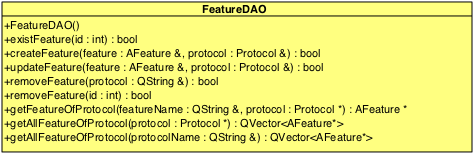
\includegraphics[scale=1]{./Content/Immagini/model/FeatureDAO.png}
			\caption{Diagramma classe \textsl{FeatureDAO}}
			\label{cl_featuredao}
\end{figure}
\paragraph{Descrizione \\}
Classe che rappresenta l'oggetto incaricato di operare con la tabella Feature\g{} del database.

\paragraph{Utilizzo\\}
La classe verrà utilizzata dal core quando dovrà salvare nel database, o recuperare da esso informazioni riguardanti le feature\g{} create dall'utente o utilizzate da \project.

\paragraph{Classi ereditate\\}
	\begin{itemize}
	\item \hyperref[speadatabase]{Romeo::Model::Util::DAO::ADatabase}.
	\end{itemize}
	
\paragraph{\textcolor{black}{Metodi\\}}
	\begin{itemize}
		\item \color{blue}\verb! + FeatureDAO()!\\
		\color{black}
		\subparagraph{Descrizione:} costruttore pubblico che richiama il costruttore della superclasse in modo da stabilire una connessione con il database.
		
		\item \color{blue}\verb!+ existFeature(id : int) : boolean!\\
		\color{black}
		\subparagraph{Desrizione:} metodo che controlla se esiste già un algoritmo con l'id passato.
		\subparagraph{Argomenti}
			\begin{itemize}
				\item \color{blue}\verb!id : int!\\
				\color{black}L'id della feature da centrare.
			\end{itemize}
		\subparagraph{Note}
			\begin{itemize}
				\item Il metodo deve essere marcato costante.
			\end{itemize}
			
		\item \color{blue}\verb!+ createFeature(feature :  AFeature*, protocol:  Protocol*): boolean!\\
		\color{black}
		\subparagraph{Descrizione:} metodo pubblico che aggiunge nel database una nuova Feature\g{} passata come parametro e simultaneamente la associa al \protocol{} passato come parametro. Ritorna true se l'inserimento avviene correttamente.
		\subparagraph{Argomenti}
			\begin{itemize}
				\item\color{RoyalPurple} \verb!feature :  AFeature*! \\ 
				\color{black}Puntatore all'oggetto \textsl{AFeature} che deve essere aggiunto nel database;
				
				\item \verb!protocol: Protocol*! \\ 
				\color{black}Puntatore all'oggetto \textsl{Protocol} a cui deve essere aggiunta la feature\g{}.
			\end{itemize}
			
		\item \color{blue}\verb! + updateFeature(feature : AFeature &, protocol : Protocol &) : boolean!\\
		\color{black}
		\subparagraph{Descrizione:} metodo che aggiorna una feature\g{} presente nel database.
		\subparagraph{Argomenti}
			\begin{itemize}
				\item \color{RoyalPurple}\verb!feature : AFeature &!\\
				\color{black}Rappresenta la feature\g{} da aggiornare;
				
				\item \color{RoyalPurple}\verb!protocol : Protocol &!\\
				\color{black}Rappresenta il Protocol\g{} assocaito alla feature\g{}.
			\end{itemize}
			
		\item \color{blue}\verb! + removeFeature(protocol : const QString &): boolean!\\
		\color{black} 
		\subparagraph{Descrizione:} metodo pubblico che rimuove nel database tutte le Feature\g{} membre del \protocol{} avente il nome passato come parametro. Ritorna true se l'eliminazione va a buon fine.
		\subparagraph{Argomenti}
			\begin{itemize}
				\item \color{RoyalPurple}\verb!protocol : const QString &! \\ 
				\color{black}Nome del Protocol di cui si vogliono eliminare le feature\g{}.
			\end{itemize}
			
		\item \color{blue}\verb! +removeFeature(id : const int) : boolean!\\
		\color{black}
		\subparagraph{Descrizione:} metodo pubblico che rimuove dal database la Feature\g{} avente l'id passato.
		Ritorna \verb!true! se l'eleiminazione va a buon fine.
		\subparagraph{Argomenti}
			\begin{itemize}
				\item \color{RoyalPurple}\verb!id : const int)!\\
				\color{black}Rappresenta l'id della feature\g{} che si vuole eliminare.
			\end{itemize}
			
		\item \color{blue}\verb!+ getFeatureOfProtocol(featureName : const QString &,!\\
									\verb! protocol : Protocol *) : AFeature *!\\
		\color{black} 
		\subparagraph{Descrizione:} metodo pubblico che ritorna un puntatore ad un oggetto di tipo \textsl{AFeature} che rappresenta la feature\g{} avente il nome passato come parametro e facente parte del \protocol{}.
		\subparagraph{Argomenti}
			\begin{itemize}
				\item \color{RoyalPurple}\verb!featureName : const QString &! \\
				\color{black} Riferimento al nome della feature\g{} che si vuole cercare;
				
				\item \color{RoyalPurple}\verb!protocol : const Protocol*! \\
				\color{black}Puntatore ad un oggetto di tipo \protocol{} nel quale si vuole cercare una Feature\g{} avente il nome passato come parametro.
			\end{itemize}
			
		%GETALLFEATUREOFPROTOCOL
		\item \color{blue}\verb!+ getAllFeatureOfProtocol(protocol : Protocol*): QVector<AFeature*>!
		\color{black} 
		\subparagraph{Descrizione:} metodo pubblico che ritorna un \textsl{QVector} di puntatori ad oggetti di tipo \textsl{AFeature}, esso contiene tutte le feature\g{} facenti parte del \protocol{} passato come parametro.
		\subparagraph{Argomenti}
			\begin{itemize}
			\item \color{RoyalPurple}\verb!protocol : const Protocol*! \\
			\color{black}Puntatore ad un oggetto di tipo \protocol{}, identifica il \protocol{} di cui si vogliono ottenere le feature\g{}.
			\end{itemize}

		
		%GETALLFEATUREOFPROTOCOL
		\item \color{blue}\verb!+ getAllFeatureOfProtocol(protocolName : const QString &): QVector<AFeature*>!
		\color{black} 
		\subparagraph{Descrizione:} metodo pubblico che ritorna un QVector di puntatori ad oggetti di tipo AFeature, esso contiene tutte le feature\g{} facenti parte del \protocol{} avente il nome uguale alla QString passata come parametro.
		\subparagraph{Argomenti}
		\begin{itemize}
			\item \verb!protocolName : const QString &! \\ 
			\color{black}Riferimento all'oggetto di tipo QString che rappresenta il nome del \protocol{} del quale si vogliono ottenere le feature\g{}.
		\end{itemize}
		
	\end{itemize}

\pagebreak
\color{black}
%%%%%%%%%%%%%%%%%%%%
%     CLASSE GROUPDAO
%%%%%%%%%%%%%%%%%%%%%%%

\subsubsection{GroupDAO(class)}
\label{spegroupdao}
\begin{figure}[!h]
\centering
			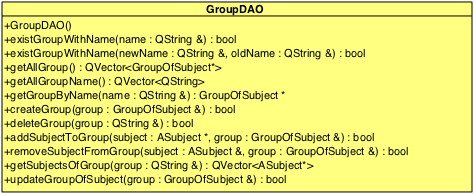
\includegraphics[scale=1]{./Content/Immagini/model/GroupDAO.png}
			\caption{Diagramma classe \textsl{GroupDAO}}
			\label{cl_groupdao}
\end{figure}

\paragraph{Descrizione \\}
Classe che rappresenta l'oggetto incaricato di operare con la tabella GroupOfSubject del database.

\paragraph{Utilizzo\\}
La classe verrà utilizzata dal core quando dovrà salvare nel database, o recuperare da esso informazioni riguardanti i gruppi di \subject{} creati dall'utente o utilizzati da \project.

\paragraph{Classi ereditate\\}
\begin{itemize}
\item \hyperref[speadatabase]{Romeo::Model::Util::DAO::ADatabase}.
\end{itemize}

\paragraph{\textcolor{black}{Metodi\\}}
	\begin{itemize}
		\item \color{blue}\verb! + GroupDAO()!\\
		\color{black}
		\subparagraph{Descrizione:} costruttore pubblico che richiama il costruttore della superclasse in modo da stabilire una connessione con il database. \\
		
		\item \color{blue}\verb! + existGroupWithName(name : const QString &): boolean!
		\color{black} 
		\subparagraph{Descrizione:} metodo pubblico che controlla se all'interno del database è presente un gruppo di \subject{} aventi il nome passato come parametro. In caso affermativo il metodo ritorna true, altrimenti false.\\
		\subparagraph{Argomenti}
			\begin{itemize}
				\item \color{RoyalPurple}\verb!name : const QString &! \\ 
				\color{black}Riferimento ad un oggetto \textsl{QString} che rappresenta il nome del Gruppo di Subject\g{} del quale si vuole controllare la presenza nel database.
			\end{itemize}
	
		\item \color{blue}\verb!+ getAllGroup(): QVector<GroupOfSubjec*>!
		\color{black} 
		\subparagraph{Descrizione:} metodo pubblico che ritorna un \textsl{QVector} di puntatori ad oggetti di tipo \textsl{GroupOfSubject}, i quali rappresentano tutti i gruppi di subject presenti nel database.

		
		\item \color{blue}\verb!+ getAllGroup(): QVector<QString>!
		\color{black} 
		\subparagraph{Descrizone:} metodo pubblico che ritorna un \textsl{QVector} di oggetti di tipo \textsl{QString}, i quali rappresentano il nome di ogni gruppo di subject\g{} presente nel database.
		
		\item \color{blue}\verb!+ getGroupByName(name : const QString &): GroupOfSubject*!
		\color{black} 
		\subparagraph{Descrizione:} metodo pubblico che ritorna un puntatore ad un oggetto \textsl{GroupOfSubject}, il quale rappresenta il gruppo di \subject{} avente il nome passato come parametro al metodo, recuperato dal database.
		\subparagraph{Argomenti}
			\begin{itemize}
				\item \color{RoyalPurple}\verb!name : const QString &! \\ 
				\color{black}
				Riferimento ad un oggetto di tipo \textsl{QString}, il quale rappresenta il nome del gruppo di \subject{} che si vuole recuperare dal database.
			\end{itemize}
			
			\item  \color{blue}\verb!+ createGroup(group :const GroupOfSubject &): boolean!
			\color{black}
			\subparagraph{Descrizione:} metodo pubblico che aggiunge nel database un nuovo gruppo di \subject{} passato come parametro. Ritorna true se l'operazione è andata a buon fine, false altrimenti.
			\subparagraph{Argomenti}
			\begin{itemize}
				\item\color{RoyalPurple} \verb!group : const GroupOfSubject &! \\ 
				\color{black}Riferimento al gruppo di \subject{} che si vuole inserire nel database
			\end{itemize}

			\item  \color{blue}\verb!+ deleteGroup(group : const QString &): boolean!\\
			\color{black}
			\subparagraph{Descrizione:} metodo pubblico che elimina dal database un gruppo di \subject{} avente il nome uguale alla QString passata come parametro. Esso ritorna true se l'operazione va a buon fine, false altrimenti.
			\subparagraph{Argomenti}
			\begin{itemize}
				\item \verb!group : const QString &! \\ Riferimento ad un oggetto di tipo \textsl{QString} il quale rappresenta il nome del gruppo di \subject{} da eliminare.
			\end{itemize}
			
			\item \color{blue}\verb! + addSubjectToGroup(subject : ASubject*, group : const GroupOfSubject &): boolean!
			\color{black} 
			\subparagraph{Descrizione:} metodo pubblico che aggiunge un \subject{}, il quale viene passato come parametro, ad un gruppo di \subject{}, anch'esso passato come parametro. Esso ritorna true se l'operazione va a buon fine, false altrimenti.
			\subparagraph{Argomenti}
			\begin{itemize}
				\item \color{RoyalPurple}\verb!subject : ASubject*! \\ 
				\color{black}Puntatore ad un oggetto di tipo \textsl{ASubject}, il quale rappresenta il \subject{} da aggiungere al gruppo;
				
				\item \color{RoyalPurple}\verb!group : const GroupOfSubject &! \\ 
				\color{black}Riferimento ad un oggetto di tipo \textsl{GroupOfSubject}, il quale rappresenta il gruppo a cui aggiungere il \subject{}.
			\end{itemize}

			\item \color{blue}\verb! + removeSubjectFromGroup(subject : ASubject*, group : const GroupOfSubject &): boolean!
			\color{black} 
			\subparagraph{Descrizione:} metodo pubblico che rimuove un \subject{}, il quale viene passato come parametro, da un gruppo di \subject{}, anch'esso passato come parametro. Esso ritorna true se l'operazione va a buon fine, false altrimenti.
			\subparagraph{Argomenti}
			\begin{itemize}
				\item \color{RoyalPurple}\verb!subject : const ASubject*! \\ 
				\color{black}Puntatore ad un oggetto di tipo \textsl{ASubject}, il quale rappresenta il \subject{} da rimuovere dal gruppo;
				
				\item \color{RoyalPurple}\verb!group : const GroupOfSubject &! \\ 
				\color{black}Riferimento ad un oggetto di tipo \textsl{GroupOfSubject}, il quale rappresenta il gruppo da cui rimuovere il \subject{}.
			\end{itemize}

			
			\item  \color{blue}\verb!+ getSubjectOfGroup(group : const QString &): QVector<ASubject*>!
			\color{black}
			\subparagraph{Descrizione:} metodo pubblico che ritorna un QVector di puntatori ad oggetti di tipo \textsl{ASubject}, i quali rappresentano tutti i \subject{} che sono membri del gruppo di \subject{} passato come parametro.
			\subparagraph{Argomenti}
			\begin{itemize}
				\item \color{RoyalPurple}\verb!group : const QString &! \\
				\color{black}Riferimento ad un oggetto di tipo \textsc{QString}, il quale rappresenta il nome del gruppo di cui ottenere i membri.
			\end{itemize}
			
			\item \color{blue}\verb! + updateGroupOfSubject(GroupOfSubject & : group) : boolean!\\
			\color{black}
			\subparagraph{Descrizione:} metodo che esegue l'aggiornamento di un gruppo di subject\g{}.
			Il metodo ritorna un booleano che indica se l'operazione è andata a buon fine.
			\subparagraph{Argomenti}
				\begin{itemize}
					\item \color{RoyalPurple}\verb!GroupOfSubject & : group)!\\
					\color{black}Il gruppo di subject\g{} da aggiornare.
				\end{itemize}

	\end{itemize}

\color{black}
%%%%%%%%%%%%%%%%%%%%
%     CLASSE PROTOCOLDAO
%%%%%%%%%%%%%%%%%%%%%%%
\pagebreak
\subsubsection{ProtocolDAO(class)}
\label{speprotocoldao}
\begin{figure}[!h]
\centering
			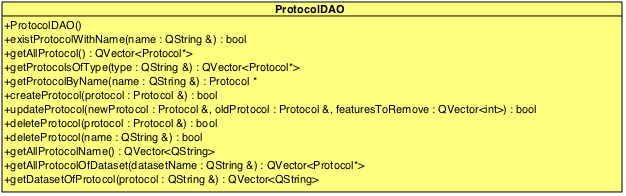
\includegraphics[scale=0.8]{./Content/Immagini/model/ProtocolDAO.png}
			\caption{Diagramma classe \textsl{ProtocolDAO}}
			\label{cl_protocoldao}
\end{figure}

\paragraph{Descrizione \\}
Classe che rappresenta l'oggetto incaricato di operare con la tabella \protocol{} del database.
\paragraph{Utilizzo\\}
La classe verrà utilizzata dal core quando dovrà salvare nel database, o recuperare da esso informazioni riguardanti i \protocol{} creati dall'utente o utilizzati da \project.
\paragraph{Classi ereditate\\}
\begin{itemize}
\item \hyperref[speadatabase]{Romeo::Model::Util::DAO::ADatabase}.
\end{itemize}

\paragraph{\textcolor{black}{Metodi\\}}
\begin{itemize}
	\item \color{blue}\verb!+ ProtocolDAO()!
	\color{black} 
	\subparagraph{Descrizione:} costruttore pubblico che richiama il costruttore della superclasse in modo da stabilire una connessione con il database.
	
	\item \color{blue}\verb!+ existProtocolWithName(name : const QString &): boolean!
	\color{black} 
	\subparagraph{Descrizione:} metodo pubblico che controlla se all'interno del database è presente un \protocol{} avente il nome passato come parametro. In caso affermativo il metodo ritorna true, altrimenti false.
	\subparagraph{Argomenti}
	\begin{itemize}
		\item \color{RoyalPurple}\verb!name : const QString &! \\ 
		\color{black}Riferimento ad un oggetto \textsl{QString} che rappresenta il nome del \protocol{} del quale si vuole controllare la presenza nel database.
	\end{itemize}
	
	\item \color{blue}\verb!+ getAllProtocol(): QVector<Protocol*>!\\
	\color{black} 
	\subparagraph{Descrizione:} metodo pubblico che ritorna un \textsl{QVector} di puntatori ad oggetti di tipo \protocol{}, i quali rappresentano tutti i \protocol{} presenti nel database.
	
	\item \color{blue}\verb! + getProtocolsOfType(type : QString &) : QVector<Protocol*>!
	\color{black}
	\subparagraph{Descrizione:} metodo che ritorna un vettore di oggetti \textsl{Protocol}, contenente tutti i Protocol\g{} di un determinato tipo (2D, 2D-T, 3D, 3D-t).
	\subparagraph{Argomenti}	
		\begin{itemize}
			\item \color{RoyalPurple}\verb!type : QString &!\\
			\color{black}Tipo dei Protocol\g{} che si vogliono ottenere.
		\end{itemize}
		
	\item \color{blue}\verb!+ getProtocolByName(name : const QString &): Protocol*!
	\color{black} 
	\subparagraph{Descrizione:} metodo pubblico che ritorna un puntatore ad un oggetto di tipo \protocol{}, il quale rappresenta il \protocol{} avente il nome uguale alla QString passata come parametro, recuperato dal database.
	\subparagraph{Argomenti}
		\begin{itemize}
			\item \color{RoyalPurple}\verb!name : const QString &! \\ 
			\color{black}Riferimento ad un oggetto di tipo \textsl{QString} che rappresenta il nome del \protocol{} da cercare nel database.
		\end{itemize}
		
	\item \color{blue}\verb!+ createProtocol(protocol : const Protocol &): boolean!
	\color{black} 
	\subparagraph{Descrizione:} metodo pubblico che consente l'inserimento nel database, del \protocol{} passato come parametro. Esso ritorna true se l'operazione va a buon fine, false altrimenti.
	\subparagraph{Argomenti}
	\begin{itemize}
		\item \color{RoyalPurple}\verb!protocol : const Protocol &! \\ 
		\color{black}Riferimento ad un oggetto di tipo \protocol{}, il quale rappresenta il \protocol{} da inserire nel database.
	\end{itemize}

	\item \color{blue}\verb! + updateProtocol(newProtocol : Protocol &, oldProtocol : Protocol &, !\\
								\verb!featuresToRemove : QVector<int>) : boolean!
	\color{black}
	\subparagraph{Descrizione:} metodo che aggiorna un Protocol\g{}.
	\subparagraph{Argomenti}
		\begin{itemize}
			\item \color{RoyalPurple}\verb!newProtocol : Protocol &!\\
			\color{black}Protocol\g{} con le nuove informazioni;
			
			\item \color{RoyalPurple}\verb!oldProtocol : Protocol &!\\
			\color{black}Vecchio Protocol\g{} da aggiornare;
			
			\item \color{RoyalPurple}\verb!featuresToRemove : QVector<int>!\\
			\color{black}Lista di feature\g{} da rimuovere.
		\end{itemize}
		
	\item \color{blue}\verb! + deleteProtocol(protocol : const Protocol &): boolean!\\
	\color{black}
	\subparagraph{Descrizione:} metodo pubblico che consente l'eliminazione dal database, del \protocol{} passato come parametro. Esso ritorna true se l'operazione va a buon fine, false altrimenti.
	\subparagraph{Argomenti:}
	\begin{itemize}
			\item\color{RoyalPurple} \verb!protocol : const Protocol &! \\
			\color{black}Riferimento ad un oggetto di tipo \protocol{}, il quale rappresenta il \protocol{} da rimuovere dal database.
	\end{itemize}
	
	\item \color{blue}\verb! + getAllProtocolName() : QVector<QString>!\\
	\color{black}
	\subparagraph{Descrizione:} metodo pubblico che ritorna un vettore di oggetti \textsl{QString} contenente l'elenco dei nomi dei vari Protocol\g{} esistenti.
	
	\item \color{blue}\verb!+ getAllProtocolOfDataset(datasetName : const QString &): QVector<Protocol*>!
	\color{black} 
	\subparagraph{Descrizione:} metodo pubblico che ritorna un QVector di puntatori ad oggetti di tipo \protocol{}, i quali rappresentano tutti i \protocol{} che sono membri del \dataset{} avente il nome uguale al parametro passato.
	\subparagraph{Argomenti}
	\begin{itemize}
		\item\color{RoyalPurple} \verb!datasetName : const QString &! \\ 
		\color{black}Riferimento ad un oggetto di tipo \textsl{QString}, il quale rappresenta il nome del \dataset{} del quale ottenere i \protocol{}.
	\end{itemize}
	
	\item \color{blue}\verb! + getDatasetOfProtocol(protocol : const QString &) : QVector<QString>!
	\color{black}
	\subparagraph{Descrizione:} metodo pubblico che ritorna un QVector di puntatori ad oggetti di tipo QString contentente i nomi dei dataset associati col Protocol\g{} passato.
	\subparagraph{Argomenti}
		\begin{itemize}
			\item \color{RoyalPurple}\verb!protocol : const QString &!\\
			\color{black}Nome del protocol\g{} di cui si vogliono conoscere i dataset\g{} associati.
		\end{itemize}

\end{itemize}














\pagebreak
%%%%%%%%%%%%%%%%%%%%
%     CLASSE SUBJECTDAO
%%%%%%%%%%%%%%%%%%%%%%%

\subsubsection{SubjectDAO(class)}
\label{spesubjectdao}
\begin{figure}[!h]
\centering
			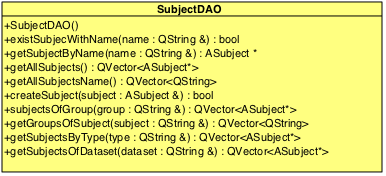
\includegraphics[scale=1]{./Content/Immagini/model/SubjectDAO.png}
			\caption{Diagramma classe \textsl{SubjectDAO}}
			\label{cl_subjectdao}
\end{figure}
\paragraph{Descrizione \\}
Classe che rappresenta l'oggetto incaricato di operare con la tabella \subject{} del database.
\paragraph{Utilizzo\\}
La classe verrà utilizzata dal core quando dovrà salvare nel database, o recuperare da esso informazioni riguardanti i \subject{} creati dall'utente o utilizzati da \project.
\paragraph{Classi ereditate\\}
\begin{itemize}
\item \hyperref[speadatabase]{Romeo::Model::Util::DAO}.
\end{itemize}
\paragraph{\textcolor{black}{Metodi\\}}
\begin{itemize}
	\item\color{blue}\verb!+SubjectDAO()!
	\color{black} 
	\subparagraph{Descrizione:} costruttore pubblico che richiama il costruttore della superclasse in modo da stabilire una connessione con il database.
	
	\item \color{blue}\verb!+ existSubjectlWithName(name : const QString &): boolean!
	\color{black} 
	\subparagraph{Descrizione:} metodo pubblico che controlla se all'interno del database è presente un \subject{} avente il nome passato come parametro. In caso affermativo il metodo ritorna true, altrimenti false.\\
	\subparagraph{Argomenti:}
	\begin{itemize}
		\item \color{RoyalPurple}\verb!name : const QString &! \\
		\color{black} Riferimento ad un oggetto \textsl{QString} che rappresenta il nome del \subject{} del quale si vuole controllare la presenza nel database.
	\end{itemize}
	\subparagraph{Note}
		\begin{itemize}
			\item Il metodo deve esseere marcato come costante.
		\end{itemize}
	

	\item\color{blue}\verb!+ getSubjectByName(name : const QString &): ASubject*!
	\color{black} 
	\subparagraph{Descrizione:} metodo pubblico che ritorna un puntatore ad un oggetto \textsl{ASubject}, il quale rappresenta il \subject{} avente il nome passato come parametro al metodo, recuperato dal database.
	\subparagraph{Argomenti}
	\begin{itemize}
		\item \color{RoyalPurple}\verb!name : const QString &! \\ 
		\color{black}Riferimento ad un oggetto di tipo QString, il quale rappresenta il nome del \subject{} che si vuole recuperare dal database.
	\end{itemize}
	\subparagraph{Note}
			\begin{itemize}
				\item Il metodo deve esseere marcato come costante.
			\end{itemize}
			
	\item \color{blue}\verb! + getAllSubject(): QVector<ASubject*>!
	\color{black} 
	\subparagraph{Descrizione:} metodo pubblico che ritorna un \textsl{QVector} di puntatori ad oggetti di tipo \textsl{ASubject}, i quali rappresentano tutti i \subject{} presenti nel database.
	\subparagraph{Note}
			\begin{itemize}
				\item Il metodo deve esseere marcato come costante.
			\end{itemize}
	
	\item\color{blue}\verb!+ getAllSubjectName(): QVector<QString>!
	\color{black} 
	\subparagraph{Descrizione:} metodo pubblico che ritorna un \textsl{QVector} di oggetti di tipo \textsl{QString}, i quali rappresentano il nome di ogni Subject\g{} presente nel database.
	\subparagraph{Note}
			\begin{itemize}
					\item Il metodo deve esseere marcato come costante.
			\end{itemize}
			
	
	\item \color{blue}\verb!+ createSubject(subject : const ASubject &): boolean!
	\color{black} 
	\subparagraph{Descrizione:} metodo pubblico che aggiunge nel database un nuovo \subject{} passato come parametro. Esso ritorna true se l'operazione va a buon fine, false altrimenti.
	\subparagraph{Argomenti}
	\begin{itemize}
	\item \color{RoyalPurple}\verb!subject : const ASubject &! \\ 
	\color{black}Riferimento al \subject{} che si vuole inserire nel database.
	\end{itemize}
	
	\item \color{blue}\verb!+ subjectsOfGroup(group : const QString &): QVector<ASubject*>!
	\color{black} 
	\subparagraph{Descrizione:} metodo pubblico che ritorna un \textsl{QVector} di puntatori ad oggetti di tipo \textsl{ASubject}, i quali rappresentano i \subject{} che fanno parte del gruppo di \subject{} avente il nome uguale alla \textsl{QString} passata come parametro.
	\subparagraph{Argomenti}
	\begin{itemize}
		\item \color{RoyalPurple}\verb!group : const QString &! \\ 
		\color{black}Riferimento ad un oggetto di tipo \textsl{QString} che rappresenta il nome del gruppo del quale si vogliono ricavare i \subject{}
	\end{itemize}
	
		\subparagraph{Note}
				\begin{itemize}
					\item Il metodo deve esseere marcato come costante.
				\end{itemize}
	
	\item\color{blue}\verb!+ getGroupOfSubject(subject : const QString &): QVector<GroupOfSubject*>!
	\color{black} 
	\subparagraph{Descrizione:} metodo pubblico che ritorna un \textsl{QVector} di puntatori ad oggetti di tipo \textsl{GroupOfSubject}, i quali rappresentano i gruppi di \subject{} di cui è membro il \subject{} avente il nome uguale alla stringa passata come parametro.
	
	\textbf{Argomenti}
	\begin{itemize}
	\item \color{RoyalPurple}\verb!subject : const QString &! \\ 
	\color{black}Riferimento ad un oggetto di tipo QString che rappresenta il nome del \subject{} del quale si vogliono ricavare i gruppi a cui esso appartiene.
	\end{itemize}

		\subparagraph{Note}
				\begin{itemize}
					\item Il metodo deve esseere marcato come costante.
				\end{itemize}
				
	\item \color{blue}\verb!+ getSubjectsByType(type : const QString &): QVector<ASubject*>!
	\color{black} 
	\subparagraph{Descrizione:} metodo pubblico che ritorna un \textsl{QVector} di puntatori ad oggetti di tipo \textsl{ASubject}, i quali rappresentano i \subject{} aventi immagini del tipo passato come parametro.
	\subparagraph{Argomenti}
	\begin{itemize}
		\item \color{RoyalPurple}\verb!type : const QString &!\\
		\color{black}Riferimento ad un oggetto di tipo \textsl{QString}, il quale rappresenta il tipo dei \subject{} che si vogliono recuperare dal database.
	\end{itemize}
	\subparagraph{Note}
		\begin{itemize}
			\item Il metodo deve esseere marcato come costante.
		\end{itemize}
		
	\item \color{blue}\verb!+ getSubjectsOfDataset(dataset : const QString &) : QVector<ASubject*>!\\
	\color{black}
	\subparagraph{Descrizione:} metodo che ritorna un vettore di puntatori a oggetti \textsl{ASubject}, contenente la lista di Subject\g{} associati ad un determinato dataset\g{}.
	\subparagraph{Argomenti}
		\begin{itemize}
			\item \color{RoyalPurple}\verb!dataset : const QString &!\\
			\color{black}Nome del dataset\g{} di cui si vogliono conoscere i subject\g{} associati.
		\end{itemize}
	\subparagraph{Note}
			\begin{itemize}
				\item Il metodo deve esseere marcato come costante.
			\end{itemize}

\end{itemize}









